
\section{Einzelprozessorsysteme}

\begin{defi}{Überlappte Verarbeitung}
    Ein erstes Ziel der Parallelität war die \emph{überlappte Verarbeitung} von langsamen und schnellen Hardware-Komponenten.
\end{defi}

\begin{example}[Überlappte Verarbeitung]{Direct Memory Access}
    % TODO: https://de.wikipedia.org/wiki/Direct_Memory_Access (Quelle)
    Unter \emph{Direct Memory Access} versteht man, wenn Hardware-Komponenten selbstständig ohne Beteiligung der CPU Daten übertragen können.
    Diese Technik erlaubt anderen Komponenten ohne Umweg über die CPU direkt mit dem Arbeitsspeicher zu kommunizieren.

    Der Vorteil des DMA ist die schnellere Datenübertragung bei gleichzeitiger Entlastung des Prozessors.

    Anders als der Name vermuten lässt, ist die wesentliche Eigenschaft von Direct Memory Access nicht der Speicherzugriff, sondern dass der Datentransfer von einer anderen Komponente und nicht von der CPU selbst initiiert wird. Dabei braucht es zu keinen Speicherzugriffen zu kommen, es sind auch direkte Kommunikationen zwischen Peripheriegeräten möglich

    TODO: Grafik
\end{example}

\begin{defi}{Überlappter I/O}

    TODO: Sinnvolle Definition und Voraussetzungen

    TODO: Grafik
\end{defi}

\subsection{Cache}

\begin{defi}{Cache}
    % TODO: https://de.wikipedia.org/wiki/Cache (Quelle)
    \emph{Cache} bezeichnet einen schnellen Pufferspeicher, der (wiederholte) Zugriffe auf ein langsames Hintergrundmedium oder aufwendige Neuberechnungen zu vermeiden hilft.

    Daten, die bereits einmal geladen oder generiert wurden, verbleiben im Cache, so dass sie bei späterem Bedarf schneller aus diesem abgerufen werden können.

    Auch können Daten, die vermutlich bald benötigt werden, vorab vom Hintergrundmedium abgerufen und vorerst im Cache bereitgestellt werden (\emph{read-ahead}).

    Da es technisch aufwändig und damit meist wirtschaftlich nicht sinnvoll ist, einen Cache zu bauen, der sowohl groß als auch schnell ist, kann man mehrere Caches verwenden -- z. B. einen kleinen schnellen und einen deutlich größeren, jedoch etwas langsameren Cache (der aber immer noch viel schneller ist als der zu cachende Hintergrundspeicher).

    Damit kann man die konkurrierenden Ziele von geringer Zugriffszeit und großem Cacheumfang gemeinsam realisieren.
    Das ist wichtig für die \emph{Hit Rate}.
\end{defi}

\begin{defi}{Cachehierarchie}
    Existieren mehrere Caches, so bilden diese eine \emph{Cachehierarchie}, die Teil der Speicherhierarchie ist.

    Die einzelnen Caches werden nach ihrer Hierarchieebene (engl. \emph{level}) durchnummeriert, also Level-1 bis Level-n oder kurz L1, L2 usw.
    Je niedriger die Nummer, desto näher liegt der Cache an der (schnell) verarbeitenden Komponente;
    die niedrigste Nummer bezeichnet daher den Cache mit der schnellsten Zugriffszeit, dieser wird als erstes durchsucht.

    Enthält der L1-Cache die benötigten Daten nicht, wird der (meist etwas langsamere, aber größere) L2-Cache durchsucht usw.
    Das geschieht solange, bis die Daten entweder in einer Cacheebene gefunden (\emph{Cache Hit}) oder alle Caches ohne Erfolg durchsucht wurden (\emph{Cache Miss}).
    In letzterem Fall muss auf den langsamen Hintergrundspeicher zugegriffen werden.
\end{defi}

\begin{example}[Cachehierarchie]{IBM Power 4}
    TODO
\end{example}

\begin{example}[Cachehierarchie]{Intel Itanium}
    TODO
\end{example}

\begin{defi}[Cache]{Zugriffszeit}
    Durch die Aufteilung des L1-Cache in Daten- und Instruktions-Cache (Harvard-Architektur) können bei Pipeline-basierten Rechnern gleichzeitig neue Instruktionen zum Füllen der Pipeline geholt werden und bei der Bearbeitung der Operanden die Daten ausgelesen werden.

    Die \emph{Zugriffszeit} $t_Z$ eines Caches kann wie folgt definiert werden:
    \[
        t_Z = t_{C} + (1 - h) \cdot t_{M}
    \]
    Dabei ist $t_C$ die Zugriffszeit des Prozessors für Werte aus dem Cache, $t_M$ die für Daten aus dem Memory und $h$ die Hit-Rate.

    Wenn die Hit-Rate groß sein soll, sind sowohl ein Programm mit hoher räumlicher und zeitlicher Lokalität, sowie ein großer Cache (meist L1, L2 und L3) erforderlich.
\end{defi}

\begin{defi}{Cache Hits und Misses}
    % TODO: https://de.wikipedia.org/wiki/Cache#Organisation (Quelle)
    Den Vorgang, dass die Daten einer Anfrage an einen Cache in selbigem vorrätig sind, bezeichnet man als \emph{Cache Hit}, den umgekehrten Fall als \emph{Cache Miss}.

    Man unterscheidet zwischen folgenden Cache Misses:
    \begin{itemize}
        \item \emph{Cold Start Miss}; tritt auf beim ersten Zugriff auf einen Block nach dem Start des Programms oder dem Task-Wechsel.
        \item \emph{Capacity Miss}; tritt auf, wenn der Cache nicht alle Blocks speichern kann, die bei der Ausführung durch die CPU benötigt werden (nur bei Fully Associative Cache).
        \item \emph{Conflict Miss}; tritt auf, wenn ein Block ersetzt werden muss, der anschließend wieder benötigt wird (bei N-way Set Associative Cache).
        \item \emph{Coherence Miss}; bei Mehrprozessorsystemen.
    \end{itemize}
\end{defi}

\begin{defi}{Hit und Miss Rate}
    % TODO: https://de.wikipedia.org/wiki/Cache#Organisation (Quelle)
    Um quantitative Maßzahlen für die Bewertung der Effizienz eines Caches zu erhalten, definiert man zwei Größen.

    Die Anzahl der Anfragen, bei denen ein Cache Hit auftrat, geteilt durch die Anzahl der insgesamt an diesen Cache gestellten Anfragen bezeichnet man als \emph{Hit Rate}.
    Wie man aus der Definition leicht sehen kann, liegt diese Größe zwischen Null und Eins. Eine Hit Rate von z. B. 70 \% bedeutet, dass bei 70 \% aller Anfragen an den Cache dieser die Daten sofort liefern konnte und bei 30 \% aller Anfragen passen musste.

    Analog zur Hit Rate ist die \emph{Miss Rate} als die Anzahl der Anfragen definiert, bei denen die Daten nicht im Cache vorhanden waren geteilt durch die Anzahl der gesamten Anfragen.
    Offensichtlich gilt:
    \[
        \text{Miss Rate} = 1 - \text{Hit Rate}
    \]
\end{defi}

\begin{defi}{Cache-Assoziativität}
    Die Cache-Lines (Blöcke) eines Caches können in so genannte \emph{Sätze} zusammengefasst werden.
    Für eine bestimmte Adresse ist dann immer nur einer der Sätze zuständig.
    Innerhalb eines Satzes bedienen alle Cache-Lines also nur einen Teil aller vorhandenen Adressen.

    Im Folgenden stehe die Variable $m$ für die Gesamtanzahl der Cache-Liness und $n$ für die Anzahl der Cache-Lines pro Satz, die so genannte \emph{Assoziativität}.
    Dann besteht der Cache also aus $\frac{m}{n}$ Sätzen.
\end{defi}

\begin{defi}[Cache-Assoziativität]{Direct Mapped Cache}
    % TODO: https://en.wikipedia.org/wiki/Cache_placement_policies#Direct-mapped_cache (Quelle)
    Bei einem \emph{Direct Mapped Cache} wird jeder Block repräsentiert einen durch eigenen Satz, es gibt also so viele Sätze wie Cache-Lines.
    Somit ist für eine gegebene Adresse exakt ein Cacheblock zuständig.

    Platzieren eines Speicherblocks im Cache:
    \begin{itemize}
        \item Bestimmen der Zeilenadresse im Cache, basierend auf Adresse um Hauptspeicher
        \item Speicherblock wird entsprechend im Cache gespeichert, als Tag wird die Hauptspeicheradresse verwendet
        \item vorher gespeicherte Daten werden überschrieben
    \end{itemize}

    Suchen im Cache:
    \begin{itemize}
        \item Bestimmen der Zeilenadresse im Cache, basierend auf Adresse um Hauptspeicher
        \item Tags (Hauptspeicheradressen) werden verglichen
        \item bei gleichen Tags \emph{Cache-Hit}, sonst \emph{Cache-Miss}
        \item bei einem Cache-Miss muss der Speicherblock in Cache geladen werden
    \end{itemize}

    Vorteile des Direct Mapped Cache sind, dass nicht alle Adressen im Cache durchsucht werden müssen und das Vorgehen sehr simpel ist.

    Im Gegenzug ist die Effizienz des Caches eingeschränkt, da möglicherweise freie Cacheblöcke vorhanden sind, die nicht genutzt werden.

    \centering
    % TODO: https://diveintosystems.org/book/C11-MemHierarchy/caching.html (Quelle)
    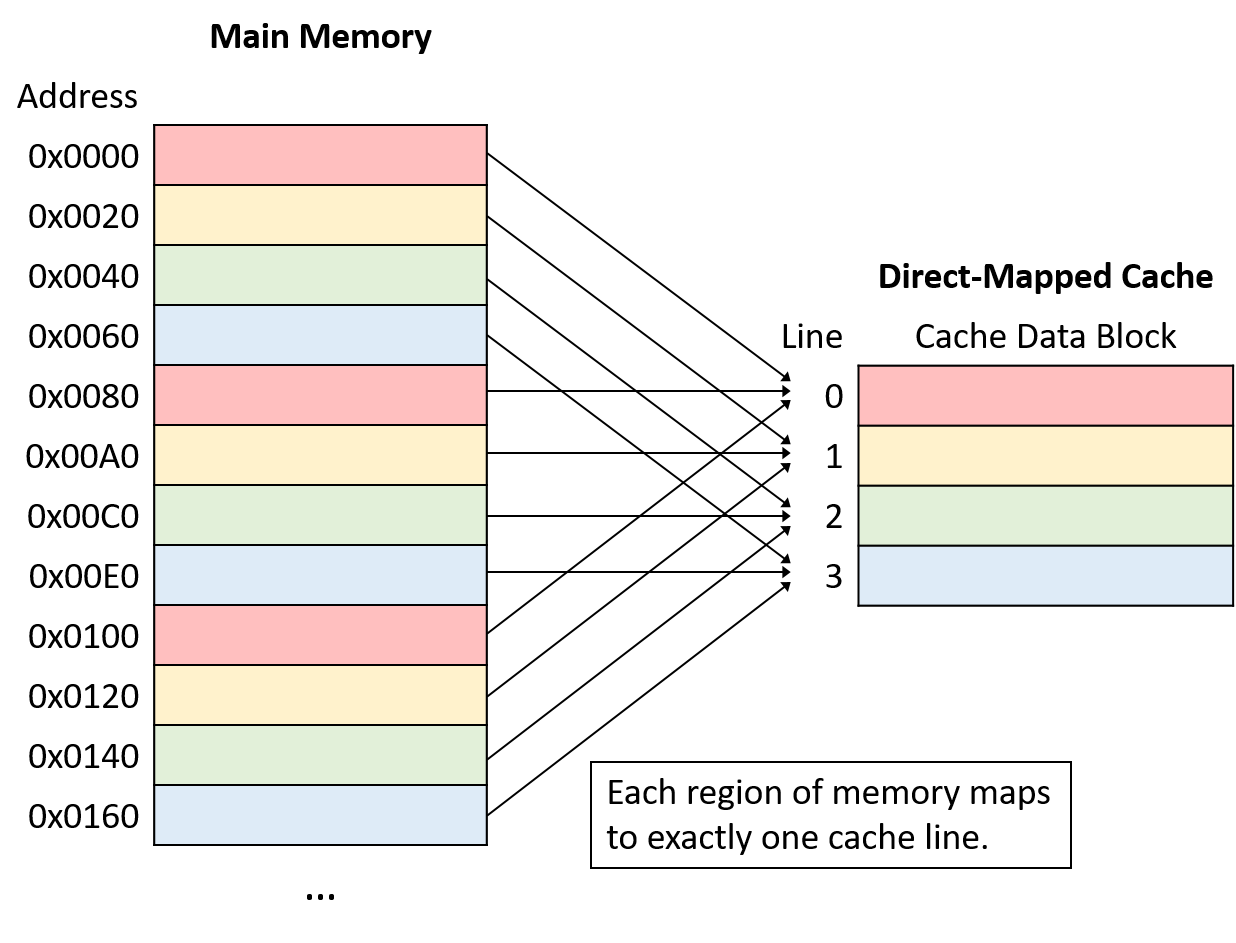
\includegraphics[width=.6\linewidth]{images/direct_mapped_cache.png}
    % 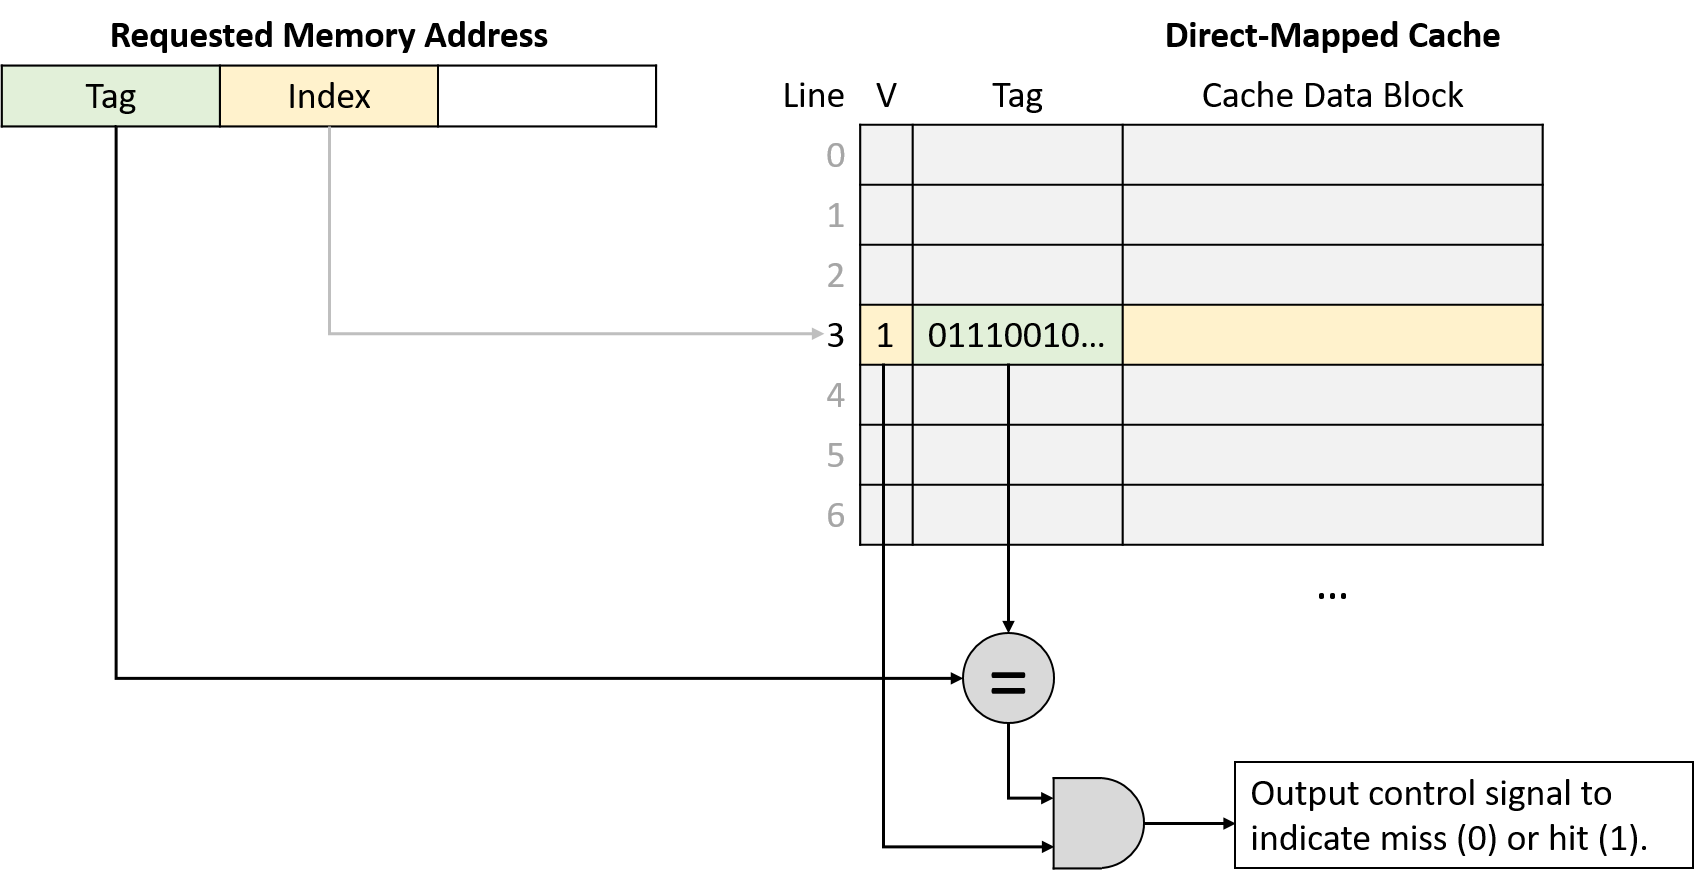
\includegraphics[width=.9\linewidth]{images/direct_mapped_cache_request.png}
\end{defi}

\begin{defi}[Cache-Assoziativität]{Fully Associative Cache}
    % TODO: https://de.wikipedia.org/wiki/Cache#Organisation (Quelle)
    Ein \emph{Fully Associative Cache} hat nur einen Satz, der alle Blöcke beinhaltet.
    Somit kann jede Adresse in jedem Cacheblock gecachet werden.

    Bei einer Anfrage an den Cache ist es daher notwendig, alle Cache-Tags zu überprüfen.
    Da Caches möglichst schnell sein müssen, wird das parallel ausgeführt, was den notwendigen Hardwareaufwand an Tag-Vergleichern vergrößert.

    Der Vorteil ist aber, dass der Cache stets Daten aufnehmen kann, solange noch ein beliebiger Cacheblock frei ist.
\end{defi}

\begin{defi}[Cache-Assoziativität]{N-way Set Associative Cache}
    % TODO: https://de.wikipedia.org/wiki/Cache#Organisation (Quelle)
    Ein \emph{N-way Set Associative Cache} reduziert Konflikte beim Zwischenlagern im Cache durch $N$ \emph{Cache-Sets}.

    Beim \emph{2-way Set Associative Cache} werden bei der Anforderung einer Hauptspeicheradresse in den beiden Cache-Sets parallel an der entsprechenden Stelle der Tag verglichen.
    Stimmt ein Tag überein, kann direkt aus dem Cache gelesen werden (\emph{Cache-Hit}).
    Sind beide Tags verschieden, muss in einem Cache-Set eine Zeile neu aus dem Hauptspeicher geladen werden (\emph{Cache-Miss}).

    Diese Cacheform stellt einen Kompromiss aus Hardwareaufwand und Effizienz des Caches dar:
    Gegenüber einem DM-Cache gewinnt man Effizienz, gegenüber einem FA-Cache spart man Hardware.

    % TODO: https://diveintosystems.org/book/C11-MemHierarchy/caching.html (Quelle)
    \centering
    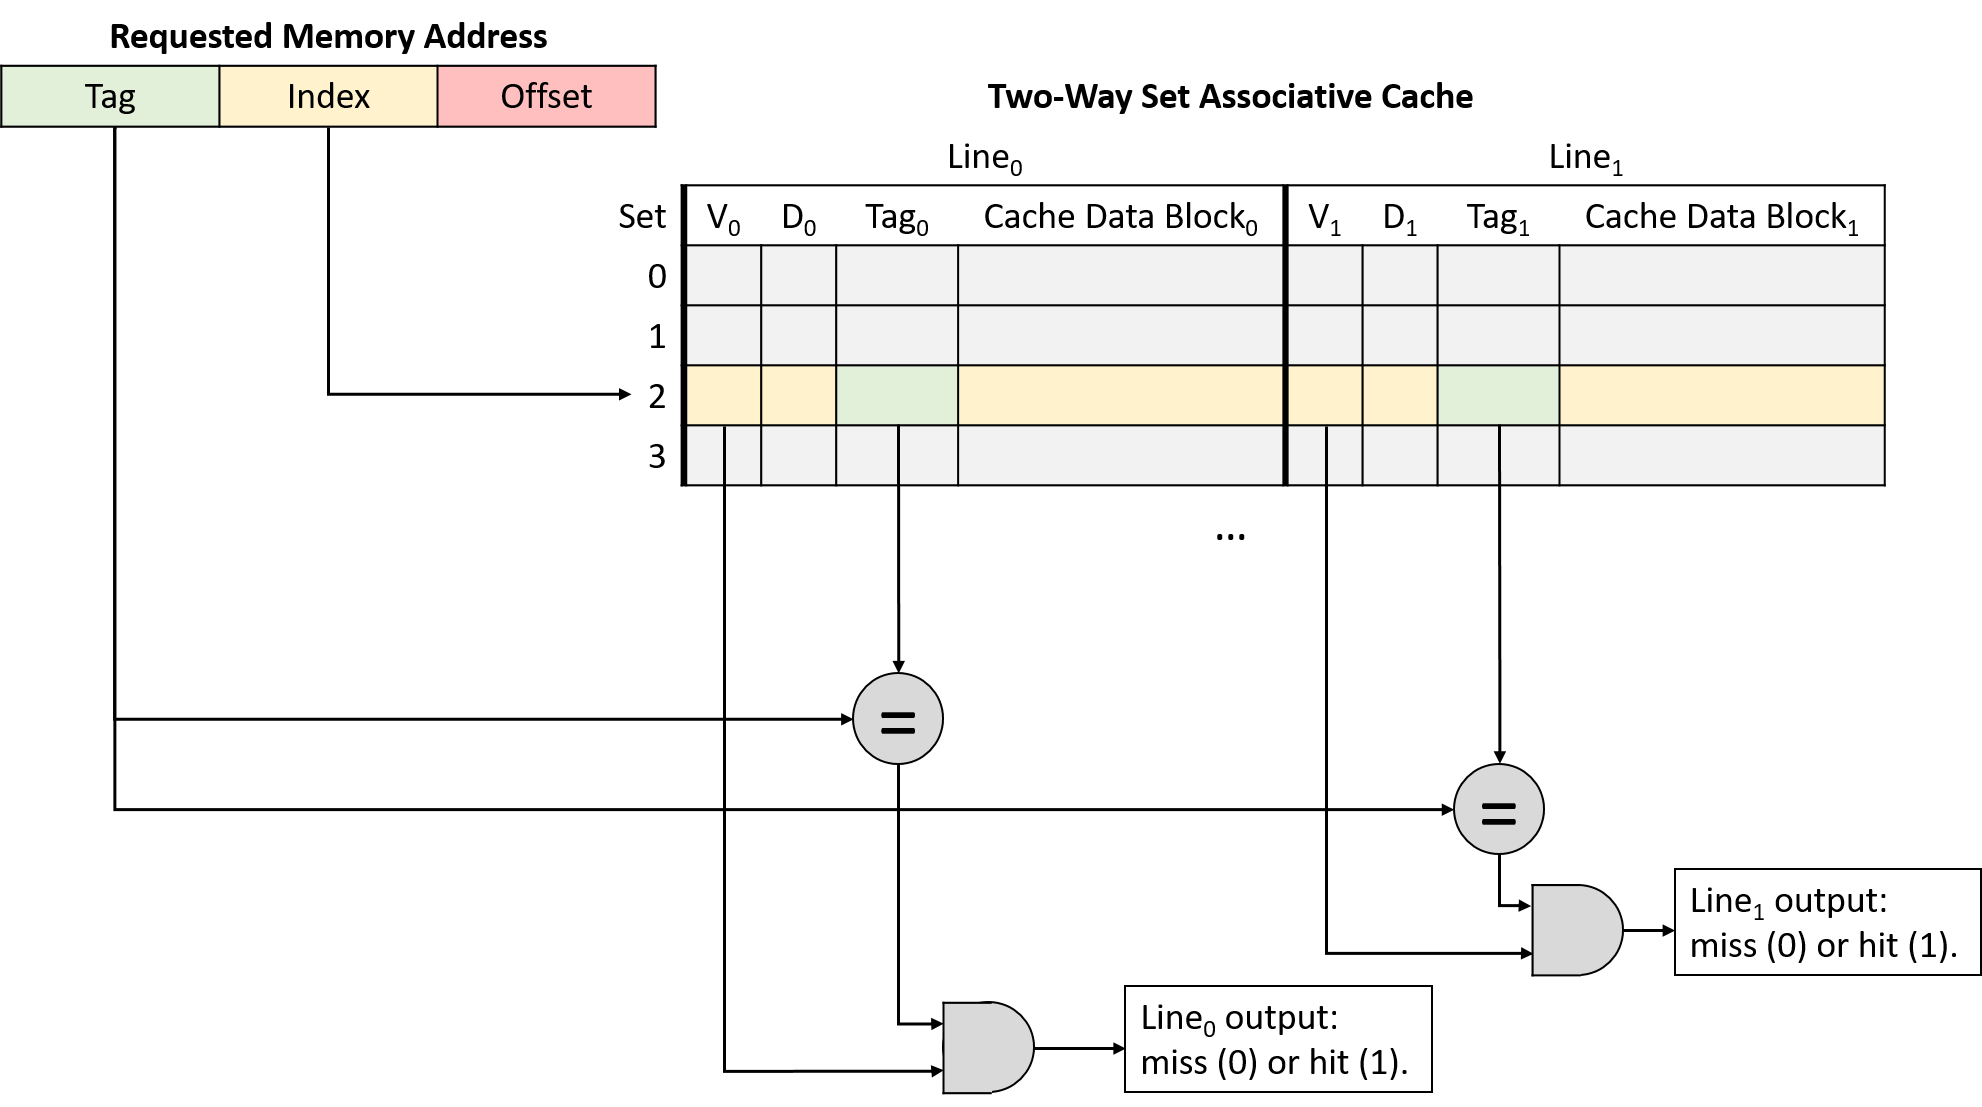
\includegraphics[width=.9\linewidth]{images/2-way_set_associative_cache_request.png}
\end{defi}

\begin{defi}{Ersetzungsstrategie}
    % TODO: https://de.wikipedia.org/wiki/Cache#Organisation (Quelle)
    Bei der Verwaltung des Caches ist es sinnvoll, immer nur die Blöcke im Cache zu halten, auf die auch häufig zugegriffen wird.
    Zu diesem Zweck gibt es verschiedene \emph{Ersetzungsstrategien}.
\end{defi}

\begin{defi}[Ersetzungsstrategie]{LRU}
    Eine häufig verwendete Ersetzungsstrategie ist die \emph{LRU} (engl. Least Recently Used), bei welcher immer der Block ausgetauscht wird, auf den am längsten nicht mehr zugegriffen wurde.

    Moderne Prozessoren (z. B. der AMD Athlon) implementieren meist eine Pseudo-LRU-Ersetzungsstrategie, die fast wie echtes LRU arbeitet, aber leichter in Hardware zu implementieren ist.
\end{defi}

\begin{defi}[Ersetzungsstrategie]{FIFO}
    Ähnlich funktioniert die \emph{FIFO-Strategie} (engl. First In First Out), bei der schlicht der jeweils älteste Eintrag verdrängt wird.
\end{defi}

\begin{defi}[Ersetzungsstrategie]{Random}
    Ebenfalls üblich ist, dass ein zufälliger Eintrag verdrängt wird (\emph{Random-Strategie}).
\end{defi}

\begin{defi}{Schreibstrategie}
    Bei einem Schreibzugriff muss generell unterschieden werden, ob ein Block bereits im Cache, oder noch ungeladen im Hauptspeicher ist.
    Es muss also eine \emph{Schreibstrategie} gewählt werden.

    Bei einem Schreibzugriff auf einen Block, der im Cache vorhanden ist, gibt es prinzipiell zwei Möglichkeiten:
    \begin{itemize}
        \item Durchgängiges Schreiben (Write-Through)
        \item Zurückkopieren (Write-Back)
    \end{itemize}

    Analog zu Obigem gibt es bei einem Schreibzugriff auf einen Block, der nicht im Cache vorhanden ist, prinzipiell ebenso zwei Möglichkeiten:
    \begin{itemize}
        \item Write-Allocate
        \item Non-Write-Allocate
    \end{itemize}

    Einige Befehlssätze enthalten Befehle, die es dem Programmierer ermöglichen, explizit anzugeben, ob zu schreibende Daten am Cache vorbeizuschreiben sind.

    Normalerweise wird entweder die Kombination Write-Back mit Write-Allocate oder Write-Through mit Non-Write-Allocate verwendet.
    Die erste Kombination hat den Vorteil, dass aufeinander folgende Schreibzugriffe auf denselben Block (Lokalitätsprinzip) komplett im Cache abgewickelt werden (bis auf den ersten Miss).
    Dies gibt im zweiten Fall keinen Vorteil, da sowieso jeder Schreibzugriff zum Hauptspeicher muss, weshalb die Kombination Write-Through mit Write-Allocate eher unüblich ist.
\end{defi}

\begin{defi}[Schreibstrategie]{Write-Through}
    % TODO: https://de.wikipedia.org/wiki/Cache#Organisation (Quelle)
    Bei \emph{Write-Through} wird der zu schreibende Block sofort in der nächsthöheren Speicherebene abgelegt.
    Damit ist die Konsistenz gesichert.

    Damit der Prozessor nicht jedes Mal warten muss, bis der Block in der nächsthöheren Speicherebene (die ja langsamer als der Cache ist) abgelegt ist, benutzt man einen Pufferspeicher (write buffer).
    Wenn dieser voll läuft, muss der Prozessor jedoch anhalten und warten.
\end{defi}

\begin{defi}[Schreibstrategie]{Write-Back}
    % TODO: https://de.wikipedia.org/wiki/Cache#Organisation (Quelle)
    Bei \emph{Write-Back} wird der zu schreibende Block nicht sofort in der nächsthöheren Speicherebene abgelegt, sondern zunächst im Cache.

    Dabei entsteht eine Inkonsistenz zwischen Cache und zu cachendem Speicher.
    Letzterer enthält somit veraltete Information.
    Erst wenn das Wort aus dem Cache verdrängt wird, wird es auch in die nächsthöhere Speicherebene geschrieben.
    Dazu bekommt jeder Cacheblock ein sogenanntes Dirty Bit, das anzeigt, ob der Block beim Ersetzen zurückkopiert werden muss.

    Das führt bei Speicherzugriff durch andere Prozessoren oder DMA-Geräte zu Problemen, weil diese veraltete Informationen lesen würden.
    Abhilfe schaffen hier Cache-Kohärenz-Protokolle wie z. B. MESI für UMA-Systeme.

    Ein Vorteil ist, dass mehrfaches Ändern eines Wertes nur im Cache durchgeführt wird.
    Allerdings kann ein Read-Miss zu einem Schreiben in den Hauptspeicher führen.
\end{defi}

\begin{bonus}[Schreibstrategie]{Write-Allocate}
    % TODO: https://de.wikipedia.org/wiki/Cache#Organisation (Quelle)
    Wie bei einem normalen Cache Miss wird bei \emph{Write-Allocate} der Block aus der nächsthöheren Speicherebene geholt.
    Die entsprechenden Bytes, die durch den Schreibzugriff geändert wurden, werden danach im gerade frisch eingetroffenen Block überschrieben.
\end{bonus}

\begin{bonus}[Schreibstrategie]{Non-Write-Allocate}
    % TODO: https://de.wikipedia.org/wiki/Cache#Organisation (Quelle)
    Bei \emph{Non-Write-Allocate} wird am Cache vorbei in die nächsthöhere Speicherebene geschrieben, ohne dass der dazugehörige Block in den Cache geladen wird.

    Das kann für manche Anwendungen Vorteile bringen, bei denen viele geschriebene Daten nie wieder gelesen werden.
    Durch die Verwendung von Non-Write-Allocate verhindert man das Verdrängen von anderen, möglicherweise wichtigen Blöcken und reduziert somit die Miss Rate.
\end{bonus}

\begin{defi}{Reduzierung der Cache Miss Rate}

\end{defi}

\begin{defi}[Reduzierung der Cache Miss Rate]{Programmierstrategien}

\end{defi}

\begin{defi}{Table-Look-Aside Buffer}

\end{defi}

\subsection{Entwicklungslinien der Prozessoren}

\begin{defi}{CISC}

\end{defi}

\begin{defi}{RISC}

\end{defi}

\begin{defi}{VLIW}

\end{defi}

\begin{defi}{EPIC}

\end{defi}